\documentclass{article}
\usepackage{comment}
\usepackage[final]{styles}
\usepackage[utf8]{inputenc} % allow utf-8 input
\usepackage[T1]{fontenc}    % use 8-bit T1 fonts
\PassOptionsToPackage{hyphens}{url}\usepackage{hyperref}       % hyperlinks
\usepackage{url}            % simple URL typesetting
\usepackage{booktabs}       % professional-quality tables
\usepackage{amsfonts}       % blackboard math symbols
\usepackage{nicefrac}       % compact symbols for 1/2, etc.
\usepackage{microtype}      % microtypography
\usepackage{amsmath}
\usepackage{amsthm}
\usepackage{amssymb}
\usepackage{tikz}
\usepackage{csquotes}
\usepackage{float}
\usepackage{graphicx}
\usepackage{wrapfig}
\usepackage{multicol}

\newcommand{\stoptocwriting}{%
  \addtocontents{toc}{\protect\setcounter{tocdepth}{-5}}}
\newcommand{\resumetocwriting}{%
  \addtocontents{toc}{\protect\setcounter{tocdepth}{\arabic{tocdepth}}}}

% \title{Harmonic Flows on Guage Equivariant Moduli Space of Connection }
% \title{Ergodic Flows on Guage Equivariant \\ Space of Connection }
% \title{Ergodic flow on Moduli\\  Space of Connections }
% \title{Attention and Energy Minimization \\ on Moduli  Space of Connections }
\title{ Emergent Attention on 
Yang-Mills \\Space of Connections}
% \title{Learning Energy Minimization on \\  Moduli Space of Connections }

% The \author macro works with any number of authors. There are two commands
% used to separate the names and addresses of multiple authors: \And and \AND.
%
% Using \And between authors leaves it to LaTeX to determine where to break the
% lines. Using \AND forces a line break at that point. So, if LaTeX puts 3 of 4
% authors names on the first line, and the last on the second line, try using
% \AND instead of \And before the third author name.

\author{%
  L. J. Pereira \\
%   \texttt{lukejoepereira@gmail.com} \\
  % examples of more authors
  % \And
  % Coauthor \\
  % Affiliation \\ consciousness
  % Address \\
  % \texttt{email} \\
  % \AND
  % Coauthor \\
  % Affiliation \\
  % Address \\
  % \texttt{email} \\
  % \And
  % Coauthor \\
  % Affiliation \\
  % Address \\
  % \texttt{email} \\
  % \And
  % Coauthor \\
  % Affiliation \\
  % Address \\
  % \texttt{email} \\
}

\begin{document}
\setlength{\abovedisplayskip}{4pt}
\setlength{\belowdisplayskip}{4pt}

\vspace{-2cm}
\maketitle

% \vspace{-1.3cm}

% \stoptocwriting
% gauge Dynamics of moduli spaces
\renewcommand{\baselinestretch}{1.0}\normalsize
\section*{Abstract}
In this paper, a process similar to hierarchical agglomerative clustering and principal component analysis is described using the formal methods of differential geometry and gauge theory that are commonly used in physical theories of electromagnetism and the strong nuclear force.
It is proposed that information organization and clustering naturally emerges from an a priori gauge symmetry of the action on the space of connections together with the stationary-action principle. In a learning model, this is achieved through pretraining of diffeomorphic mappings of neural network activity onto Lie groups, i.e. manifolds of continuous symmetries, which are further projected onto a differentiable and conformally invariant 4-dimensional manifold of connections. 
Constructing a Yang-Mills moduli space of connections allows us to cluster the vector activity of an ensemble of neural networks into islands of agreement forming a dynamic and unoriented part-whole hierarchy.
% It is claimed to be possible to avoid an a priori definition of a measure or metric on a specially organized latent space and moreover, that a lack of a well-defined metric can be used to prevent information redundancy using a conformal invariance property of the space. Instead, 
We can think of the clustering process as an intrinsic geometric flow on the connection space, namely the Ricci Yang-Mills flow.
The wedge product of configurations of differential forms located at critical points of the Yang-Mills action functional are comparable to axes of a $p$-dimensional ellipsoid formed in principal component analysis. These volumetric structures similarly cluster and reduce information to its principal components based on covariance and can be used as a generalized attention mechanism when applied to an ensemble of learning models. 
% The theoretical objects representing solutions of these flows are studied as quasiparticles and can be made physical in quantum materials or gasses. This geometric formulation of general intelligence is a naturally arising and biologically plausible model for quantum AI. 
% Moreover, fusing physical field theories with neuroscience and ML may justify introspection into the Anthropic Principle and cosmological fine-tuning. 


% \resumetocwriting
% \renewcommand{\baselinestretch}{0.65}\normalsize
\tableofcontents
% \renewcommand{\baselinestretch}{1.0}\normalsize





\newpage
\section{Overview}
These concepts will be described in later sections, this overview serves as a rough outline for those familiar with the relevant areas of mathematics and machine learning.
The moduli space of connections is constructed by quotienting the space of principal connections by a Lie structure group, generating a gauge equivariant parameter space.  
In particular, the Yang-Mills moduli space, a subset of the total connection space made of flat and irreducible connections, can be constructed to be a smooth, compact, and oriented manifold in 4 dimensions with critical points known as Yang-Mills connections or instantons. These connections minimize curvature between fibers and, from an information geometric perspective, they minimize relative entropy or KL divergence between open sets of gauge equivariant manifolds. 
This space can be used to cover the activity of a collection of neural networks, represented as trajectories on vector bundles. 
% Dynamics of attention are computed by minimizing the energy functional of the connection space.  Using instantons as sources of variational noise, we train an attention mechanism to minimize total energy of the moduli space. This process is comparable to finding stable solutions of an intrinsic flow on an undefined metric, namely a Ricci Yang-Mills flow with solutions akin to Ricci solitons that are real, non-volume preserving objects around invariant points. Stable solutions represent islands of agreement formed through consensus within a dynamic and unoriented part-whole hierarchy. 


A top-down energy-based attention mechanism, referred to as the moduli attention, can be trained on this space using sampled activity of the trajectories of underlying networks through a composition of energies. Motivated by the stationary-action principle, dynamics of attention are computed by minimizing the action functional of the connection space. The Yang-Mills action functional serves as a cost function on which inference minimizes the total energy in search of a basis of instanton connections. The connections are described using proejctive measurement given by a weighted sum or integral over differential forms. In comparison to statistical learning, this real, non-volume preserving object in the 3-dimensional space can be compared to a p-dimensional ellipsoid as found in principal component analysis, with axes that are typically formed using eigenvectors of the covariance matrix of a dataset. 
% Thus, the processes of this learning method are as follows: 
% \begin{enumerate}
%     \item Pretrain $model_1$ to learn diffeomorphic projective mappings of arbitrary neural network outputs onto open sets (i.e. sheaves) of continuous symmetry Lie group manifolds. This will later be used to sample activity of an ensemble of neural networks to project onto a Yang-Mills moduli space.
%     \item Pretrain $model_2$ to construct diffeomorphic mappings of sheaves of Lie groups onto sheaves of a smooth and continuous 4 dimensional manifold of connections. This will form the Yang mills moduli space of connection on which the output of $model_1$ is projected onto and where attention emerges.
%     \item Train an energy-based model, $model_3$ to find instanton connections with minimized curvature and maximized covariance by minimizing the Yang-Mills action functional given test data of various configurations of vector activity. This will later minimize vector activity projected by $model_2$.
%     \item Periodically, $model_1$ projects the ensemble of neural networks onto the Yang-Mills moduli space constructed by $model_2$ as $model_3$ determines the optimal configuration of instanton connections to minimize total energy. The approximate variational inference of $model_3$ produces a generative effect on the underlying neural networks inputs being sampled.
% \end{enumerate}

% \section{Methods}

% \section{Experiments}

\section{Geometry of Latent Information}

\subsection{Manifolds, Vector Bundles, Connections}
    A bundle serves as a useful mathematical object to analyse both the recursive construction of biological and artificial neurons and networks. It also provides descriptions of the geometry of latent information as manifolds that  are used for information processing and statistical learning.
    A fiber bundle formalizes the notion of one topological space (called a fiber) being parameterized by another topological space (called a base). The bundle is equipped with a group action on the fiber that represents different ways the fibers can be viewed as equivalent (Tao 2008). Bundles also have a property, known as local trivialization, allowing neighborhoods of the bundle to be computed as simple, oriented product spaces, despite the global space being unoriented or twisted.
    
    A family of fibers associated to a base can be described by defining a template fiber from which all others are diffeomorphic to. This is formalized by defining a diffeomorphic mapping that takes positional data from the entirety of the space of fibers to a base, and implicitly from one fiber to another. When the template fiber is a vector space, we get a vector bundle. 
    %Similarly, a standard template connection between fibers, known as a principal Ehresmann connection, will also exist and can be understood as a covariant directional derivative on the tangent spaces of the manifolds. 
    A Lie group has a recursive property that results from the group being a differentiable manifold of a continuous symmetry. A useful phenomenon occurs when equipping a bundle with a Lie group action; the bundle structure can be used to represent both the original vector bundle as well as a higher-level collection of mappings between their tangent spaces, in what's known as a bundle of connections. 
    

\subsection{A Priori Structure Groups}
    
    % Hebbian learning is a form of activity-dependent synaptic plasticity where correlated activation of pre- and postsynaptic neurons leads to the strengthening of the connection between the two neurons. Another central theory of cognitive neuroscience is that different parts or modules of the brain perform different functions, known as functional localization.
    % Recall, \textit{covariance} is a measure of the joint variability of two random variables and is increasingly positive when the variables tend to show similar behavior and grow increasingly negative when dissimilar. This conversion of physical synapses into a set of random variables can be described with Markov partitions and Bernoulli Schemes. 
    % At each step, the accuracy of the model naturally decrease as a result of merging imperfectly covariant random variables.
    %     However, some form of a priori covariance is necessary for maintaining information integrity through bilateral and hierarchical dynamics, i.e. to allow a connection to communicate in a general and equivariant way between modules and within their intrinsic substructures. 
    
    % \begin{wrapfigure}{r}{0.5\textwidth}
    %     \begin{center}
    %     \includegraphics[width=0.43\textwidth]{DTI-sagittal-fibers.jpg}
    %     % \caption{Fiber tracts that run through the mid-sagittal plane}
    %     \end{center}
    % \end{wrapfigure}
    
   A biological first principle of covariance arises naturally from analysis of neuronal activity, which favours functional localization and Hebbian learning.
    Moreover, cognitive networks in the brain flow in connectome-specific diffusive waves along gyrification paths, which are theorized to be caused by differential tangential growth. 
    Recall, covariance is a measure of the joint variability of a pair random variables and is increasingly positive when the pair show similar behavior and is negative when dissimilar.
     We can imagine a simple partition scheme by  assigning a Bernoulli random variable to each synapse. Then, while ``zooming out" we merge random variables together based on their covariance and locality to build a course-grained model.
    Moving from discrete random variables (i.e. synapses) to continuous fields and manifolds (i.e. EM fields), the covariant derivative between fibers of a bundle arises naturally as the principal Ehressmann connection. 
    A connection on a fiber bundle is a device that defines a notion of parallel transport on the bundle.
    % Similar to the template fiber in a bundle, the principal Ehresmann always exists as the standard connection and can be understood as a covariant directional derivative on the tangent spaces of the manifolds.
    It proves necessary to impose an a priori covariance principle to maintain integrity of information during parallel transportion in bilateral and hierarchical directions.
    Yet for a standard learning model, covariance of functionality is an a posteriori feature because the joint variability is unknown until individual modules are trained. 
    Covariance of fibers can be achieved by imposing the structure group to be Lie groups, but can also be achieved by imposing restrictions on the projection map of Riemannian manifolds without explicitly defining the structure group beforehand (Gao 2021).

    % \begin{figure}[h]
    %     \centering
    %     \includegraphics[width=5.5cm]{DTI-sagittal-fibers.jpg}
    %     % \caption{Fiber tracts that run through the mid-sagittal plane}
    % \end{figure}
    \vspace{-0.5cm}
    \begin{figure}[h]
        \centering
        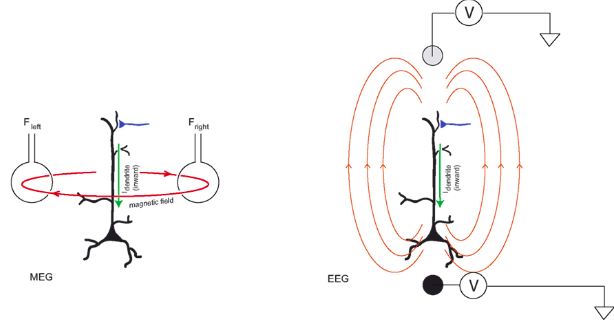
\includegraphics[width=7.5cm]{eeg-meg-neuron.png}
        \\ Diffusive magnetic (left) and electric (right) current produced by neurons
    \end{figure}
    
\subsection{Moduli Spaces and Instantons}
    With covariance established on connections, it becomes possible to perform inference using higher levels of abstraction on gauge fields. This is done by constructing a gauge equivariant bundle of connections known as a moduli space of connections, which can be further reduced to a finite dimensional manifold known as a Yang-Mills moduli space. This reduced space has local and global minima being connections with minimized energy known as Yang-Mills connections or instantons which serve as a natural choice of connection on principal and vector bundles since they minimize their curvature. From an information geometric perspective, this can be thought of as minimizing relative entropy or KL divergence between sampled trajectories of gauge equivariant manifolds. The infinitesimal form of the the KL divergence is comparable to the Fisher information metric. The gauge field strength is the curvature $F_{A}$ of the connection $A$, and the energy of the gauge field is given by the Yang–Mills action functional $YM$. With the aim of having zero or vanishing curvature, we vary parameters in search of a connection with curvature as small as possible. The Yang–Mills action functional corresponds to the $L^{2}$-norm of the curvature, and its Euler–Lagrange equations describe the critical points of this functional, either the absolute  local minima.   
    \begin{equation}
         {\displaystyle \operatorname {YM} (A)=\int _{X}\|F_{A}\|^{2}\,d\mathrm {vol} _{g}.}
    \end{equation}
    
    \subsection{Instantons as Principal Components}
    Principal Component Analysis (PCA) can serve as a motivating reference for the geometric methods proposed in this paper. PCA is commonly used to obtain lower-dimensional data while preserving as much of the data's variation as possible. The principal components of a collection of points in a real coordinate space are a sequence of $p$ unit vectors, where the $i$-th vector is the direction of a line that best fits the data while being orthogonal to the first $i-1$ vectors.  It can be shown that the principal components are eigenvectors of the data's covariance matrix. PCA can be thought of as fitting a $p$-dimensional ellipsoid to the data, where each axis of the ellipsoid represents a principal component. If some axis of the ellipsoid is small, then the variance along that axis is also small.  Similarly, a connection corresponds to the covariant directional derivitive and is considered a self-dual connection or an instanton if the curvature $2$-form is an eigenvector of the Hodge operator with eigenvalue $\pm 1$.
    

    \subsection{Instantons as Islands in Part-Whole Hierarchies}
    The GLOM model (Hinton 2021) represents part-whole hierarchies using clusters of matching vectors, known as islands of agreement, as nodes in parse tree representations within a neural network. A part-whole hierachy system consists of components that can themselves be further broken down into subcomponents. The model learns analogical reasoning by encoding parts that are not well defined or obscured. An emphasis is given on viewpoint and coordinate invariance, which allows for exchangeability within the network and is used to adapt to and generate novelty in a manner similar to creativity in humans. Comparisons can be drawn between the GLOM model and moduli attention, with vector encodings corresponding to dynamic trajectories on vector bundles, frame invariance corresponding to the gauge equivariant connection space, and islands of agreement corresponding to stable instanton solutions. Iterative consensus often does not converge in meaningful ways due to the difficulty of encoding prior understandings of desirable representations to be generated through agglomerative clustering. Using a geometric model we find that we are better able to converge to coherent clusters because of the use of an a priori structure group that imposes meaningful symmetry on the clusters and optimizes organization of information throughout the space. 
    
\section{Dynamics of Latent Information}


\subsection{Intrinsic Geometric Flows}
    \begin{wrapfigure}{r}{0.4\textwidth}
        \vspace{0.3cm}
        \centering
        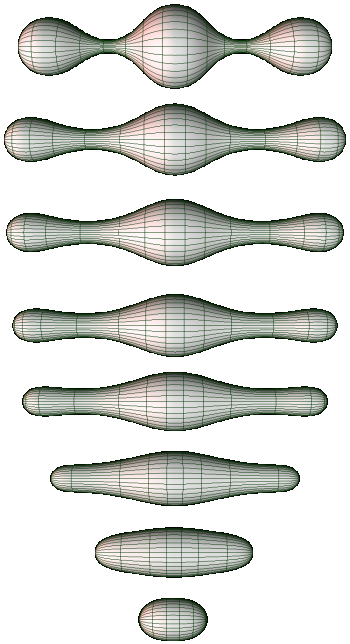
\includegraphics[scale=0.3]{ricci-flow.png}
        % \caption{Ricci flow visualization (Rubinstein, 2005)}
        \\ Ricci flow of a metric manifold (Rubinstein, 2005)
    \end{wrapfigure}
    
    We can interpret energy minimization as a geometric flow, either on the parameter space as an extrinsic flow through variational gradient descent, or on the moduli space as an intrinsic flow. A Ricci flow is an example of an intrinsic flow on the metric by which one can take an arbitrary manifold and smooth out the geometry to make it more symmetric, whereas a mean curvature flow (as found in soap films, with critical points as minimal surfaces) is an example of an extrinsic flow on an embedded manifold. The moduli attention mechanism can be understood as a mix of the two categories; manipulating both the embedded manifolds constructed from hierarchical neural networks and the moduli space of connections (or metric) itself. We can further classify it as both a variational and a curvature flow since it evolves to minimize the Yang-mills action functional which is the $L^2$ norm of curvatures. 
    % The Ricci flow, Calabi flow, and Yamabe flow all arise in similar ways. 
    Curvature flows may not necessarily preserve volume (the Calabi flow does, while the Ricci flow does not), meaning the flow may simply shrink or grow the manifold, rather than regularizing the metric. Instead of normalizing the flow by fixing the volume, we allow dissipative solutions to exist, forming a memory and compression mechanism. 

    \subsection{Ricci Yang-Mills Flow}
    
    A Ricci flow is a differential equation on the space of Riemannian metrics on $M, \mathfrak{Met}$. We can picture the Ricci flow as moving a manifold around by internal symmetries (the family of diffeomorphisms) and a uniform-in-space scaling at each time. If one works in the moduli space of $\mathfrak{Met}/ \mathfrak{Diff}$, where $\mathfrak{Diff}$ is the group of diffeomorphisms on $M$, then one allows for a family of fixed points that are metrics that flow by scaling and diffeomorphism. i.e. $g(t) = \sigma (t) \phi (t) ^* g_0$,
    where $\phi(t) :M \rightarrow M$ is a one parameter family of diffeomorphisms. 
    These are the Ricci soliton metrics. 
    In the standard quantum field theoretic interpretation of the Ricci flow in terms of the renormalization group, the parameter $t$ corresponds to length or energy rather than time.
    One can show that Ricci soliton metrics satisfy the following equation: $Rc+\mathcal{L}_X g+ 
    \frac{\epsilon}{2} g = 0$, where $X$ is the vector field generating the diffeomorphisms, and $\epsilon = -1,0,1$ corresponds to shrinking, steady, and expanding solitons respectively. If $X$ is the gradient of some function, i.e. $X=\triangledown f$, then a solution is said to be a gradient Ricci soliton. 
    Similarly, the Ricci Yang-Mills flow is a natural coupling of the Ricci flow and the Yang-Mills heat flow. It was discovered that the Ricci Yang-Mills flow is an ideal candidate for studying magnetic flows. Given a choice $h$ of metric on the Lie algebra $g$ of $G$, a one-parameter family of metrics $g_t$ on $\Sigma$ and principal connections $\mu_t$ satisfies the RYM flow if, 
    \begin{equation}
        \frac{\partial}{\partial t} g = -2 Rc \ g + F^2_\mu,  \ \ \ \ \ \ \ \ \ \ \ \ \ 
        \frac{\partial}{\partial t}\mu = -d^*_gF_\mu .
    \end{equation}
    
    \subsection{Instantons as Invariant Points}
    The stationary-action principle is a variational principle that, when applied to the action of a mechanical system, yields the equations of motion for that system. The principle states that the trajectories (i.e. the solutions of the equations of motion) are stationary points of the system's action functional.
    
    Ricci solitons and Ricci Yang-Mills solitons can be naturally associated to invariant or stationary points in metric spaces using Geometric Invariant Theory (Jablonski 2013).
    % The Ricci Yang-Mills flow is invariant under automorphisms of the principal bundle. The Ricci Yang-Mills flow preserves the set of left-invariant metrics on a Lie group.
    % It can be shown that there exists many families of Lie groups that do not admit invariant Ricci soliton metrics but admit Ricci Yang-Mills solitons, making them more reliable (though weaker) candidates for invariant points.
    Similarly, the Banach fixed-point theorem guarantees existence of a fixed point in certain metric spaces given a contractive mapping, and can be interpreted as solition solutions of a Ricci de Turck flow. A comparison can be made with the Invariant Point Attention (IPA) mechanism introduced in Alphafold 2 (Jumper 2021). The invariant point attention augments each of the standard attention queries, keys, and values with 3-D points produced in the local frame of each protein residue gas such that the final value is invariant to global rotations and translations. 
    After each attention operation and element-wise transition block, the module computes an update to the rotation and translation of each backbone frame. 
    The application of these updates within the local frame of each residue makes the overall attention and update block an equivariant operation on the residue gas.
    
    % The Banach fixed-point theorem (also known as the contraction mapping theorem or contractive mapping theorem) is an important tool in the theory of metric spaces; it guarantees the existence and uniqueness of fixed points of certain self-maps of metric spaces, and provides a constructive method to find those fixed points.

    
    % The 3-D queries and keys also impose a strong spatial/locality bias on the attention which is well-suited to iterative refinement of the protein structure. 
    


\begin{comment}

\subsection{Variational Methods in Energy-Based Models}
    \begin{figure}[H]
        \centering
        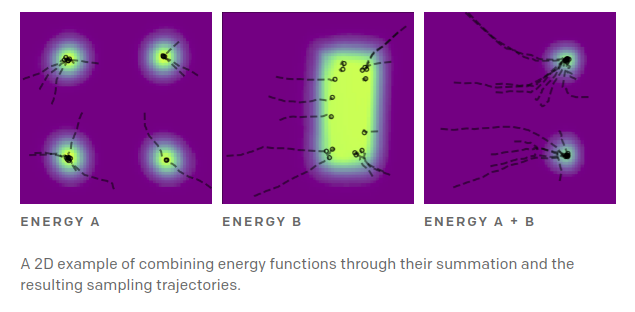
\includegraphics[width=13cm]{openai-ebm.png}
        \vspace{-0.87cm}
        \\  (Yilun, 2019)
        % \caption{Fiber tracts that run through the mid-sagittal plane}
    \end{figure}
    As underlying neural networks perform inference, their latent trajectories pass through layers of a neural network in a bottom-up manner. At the same time, a top-down variational noise is produced around the instanton solutions that best minimize energy of the total activity on the moduli space of connections. Using an energy-based model (EBM) we sample the joint distribution as a sum of each latent trajectory, corresponding to a product of experts model. This forms an attention mechanism, which we refer to as the moduli attention, and is learned on the top-down manifold while having a generative effect on underlying networks through approximate inference. This has recently been implemented using Stein Variational Gradient Descent algorithm (Jaini 2021).
    Recall, variational methods pick a family of distributions over the latent variables with their own variational parameters, $q(z_{1:m} | v)$, then attempt to find settings of the parameters that makes $q$ close to the posterior of interest. Closeness of the two distributions is measured with the KL divergence, 
    % $\displaystyle KL(q||p)=  E_q\bigg[ \log \frac{ q(z)}{p(z | x)} \bigg].$
    \begin{equation}
         \displaystyle KL(q||p)=  E_q\bigg[ \log \frac{ q(z)}{p(z | x)} \bigg].
    \end{equation}
    

         An energy function $E$ in an EBM can be thought of as an unnormalized negative log probability (LeCun 2020). 
    To convert an energy function to its equivalent probabilistic representation after normalization,
    % Recall, marginalisation is a method that sums over the possible values of one variable to determine the marginal contribution of another. 
    $P(y \mid x)$, we apply the Gibbs-Boltzmann formula with latent variables $z$ being marginalized implicitly through integration, i.e. $P(y \mid x) = \int_z P(y,z | x)$. Then,
    \begin{align*}
        P(y \mid x) &= \frac{ \int_z \exp(-\beta E(x,y,z)) }{ \int_y \int_z \exp(-\beta E(x, y, z))} 
    \end{align*}
    The derivation introduces a $\beta$ term which is the inverse of temperature $T$, so as $\beta \rightarrow \infty$ the temperature goes to zero, and we see that $\check{y} = \text{argmin}_{y} E(x,y)$. We can redefine our energy function as an equivalent function with free energy $F_\beta$,
    \begin{align*}
        F_{\infty} (x,y) &= \text{argmin}_z E(x,y,z)\\
        F_{\beta} (x,y) &= -\frac{1}{\beta} \log \int_z \exp(-\beta E(x,y,z)).
    \end{align*}
    If we have a latent variable model and want to eliminate the latent variable $z$ in a probabilistically correct way, we just need to redefine the energy function in terms of $F_\beta$,
    \begin{equation}
         P(y \mid x) = \frac{ \exp(-\beta F_\beta(x,y,z)) }{ \int_y \exp(-\beta F_\beta(x, y, z))}.
    \end{equation}
    With variational methods, instead of only minimizing the energy function with respect to $z$ we must prevent the energy function from being 0 everywhere by constraining the flexibility of the latent variable $z$. The energy function is defined as sampling $z$ randomly according to a distribution whose logarithm is the cost that links it to $z$. This distribution is commonly chosen to be a Gaussian with mean $\bar z$ which results in Gaussian noise being added to $\bar z$. The reparameterization trick is often used to allow for backpropagation during training despite the random sampling.

    
\end{comment}

% \newpage    
   

\subsection{Instantons and Self-Organized Criticality}
    Neuronal avalanches are scale-invariant neuronal population activity patterns in the cortex that are proposed to be a mechanism of cortical information processing and storage. Theory and experiments suggest neuronal avalanches allow for the formation of local and system-wide spanning neuronal groups. The condensation of instantons can describe the noise-induced chaotic phase of SOC, which maximizes connection distance while minimizing energy. A generic SOC system can be formulated as a Witten-type topological field theory (W-TFT) with spontaneously broken Becchi-Rouet-Stora-Tyutin (BRST) symmetry. There must exist regions where the BRST-symmetry is spontaneously broken by instantons, which in the context of SOC are avalanches (Ovchinnikov 2011). Stochastic neural networks have demonstrated how spontaneously broken BRST symmetry can describe SOC (Jian 2021). 
    

% \vspace{-0.3cm}
% \section{Intrinsic and Extrinsic Variational Flows}


    % $ \ \ \displaystyle KL(q||p)=  E_q\bigg[ \log \frac{ q(z)}{p(z | x)} \bigg].
    % $
    
    \subsection{Instantons and Boundaries}
    
    \begin{wrapfigure}{r}{0.4\textwidth}
        \vspace{-1.2cm}
        \centering
        
\includegraphics[scale=0.2]{Donaldson's_Theorem_cobordism.png}
        % \caption{Ricci flow visualization (Rubinstein, 2005)}
        \\ Cobordism given by Yang–Mills moduli space in Donaldson's theorem
    \end{wrapfigure}
    
    % \begin{figure}[h]
    %     \centering
    %     
\includegraphics[width=6cm]{Donaldson's_Theorem_cobordism.png}
    %     \\ Cobordism given by Yang–Mills moduli space in Donaldson's theorem
    % \end{figure}
    
    
    Moduli of Yang–Mills connections have been most studied when the dimension of the base manifold $X$ is four. Here the Yang–Mills equations admit a simplification from a second-order PDE to a first-order PDE, the anti-self-duality equations. 
    Donaldson's Theorem shows that it is possible to compactify the moduli space by cutting off cones at a reducible singularities and gluing in a copy of ${\displaystyle \mathbb {CP} ^{2}}$. Secondly, glue in a copy of $X$ itself at infinity. The resulting space is a cobordism between $X$ and a disjoint union of ${\displaystyle b_{2}(X)}$ copies of ${\displaystyle \mathbb {CP} ^{2}}$ with its orientation reversed, where $b_{2}(X)$ is the the $2$nd Betti number.
    
    \clearpage
    An instanton can be used to calculate the transition probability for a quantum mechanical particle tunneling through a potential barrier. One example of a system with an instanton effect is a particle in a double-well potential. In contrast to a classical particle, there is non-vanishing probability that it crosses a region of potential energy higher than its own energy.

    
    
    \subsection{Instantons as Quasiparticles}
    
    % \begin{comment}
    % quasiparticles and collective excitations
    % - Instantons and solitons
    
    % - Ricci solitons
    % https://math.stackexchange.com/questions/802933/ricci-soliton-geometric-meaning
    
    % - RICCI YANG-MILLS SOLITONS
    % https://arxiv.org/pdf/0907.1095.pdf
    % https://arxiv.org/pdf/2102.09538.pdf
    
    % \end{comment}
    
    % The objects representing solutions of variational flows can be studied as quasiparticles and have been made physical in quantum materials or gasses. This geometric formulation of general intelligence is a naturally arising and biologically plausible model for quantum AI. Aside from providing a computational scheme, it's worth acknowledging the philosophical implications of associating physical unified field theories with neuroscience and machine learning theory. Namely, that it  may justify further introspection into the Anthropic Principle and cosmological fine-tuning.
    
    Quasiparticles or collective excitations are emergent phenomena that encapsulate macroscopic portions of a complicated microscopic system such that the behaviour of these encapsulated parts imitate  behaviours of weakly interacting particles in a vacuum. 
    A soliton is a localized, non-dispersive solution of a nonlinear theory in Euclidean space and is a real object. Conversely, instantons are not real and only exist as solutions to the equations of motion of a quantum field theory after a Wick rotation, in which time is made imaginary. Thus, instantons are not observable, but are used to calculate and explain quantum mechanical effects that can be observed, such as tunneling. In quantum chromodynamics (QCD) instantons tunnel between the topologically different color vacua.
    
\textit{Work in Progress}


\section*{References}

\small

[1] Gao, Tingran. "The diffusion geometry of fibre bundles: Horizontal diffusion maps." Applied and Computational Harmonic Analysis 50 (2021): 147-215.
% https://arxiv.org/pdf/1602.02330.pdf

[2] Eckhard Meinrenken, "Principal bundles and connections", Lecture Notes. 
% http://www.math.toronto.edu/mein/teaching/moduli.pdf

[3] Tao, T. "What is a gauge?" (2008) https://terrytao.wordpress.com/2008/09/27/what-is-a-gauge/
% https://terrytao.wordpress.com/2008/09/27/what-is-a-gauge/

[4] Du, Yilun, and Igor Mordatch. "Implicit generation and generalization in energy-based models." arXiv preprint arXiv:1903.08689 (2019).
% https://arxiv.org/abs/1903.08689


[5] Hinton, Geoffrey. "How to represent part-whole hierarchies in a neural network." arXiv preprint arXiv:2102.12627 (2021).

[6] Hinton, Geoffrey E. "Mapping part-whole hierarchies into connectionist networks." Artificial Intelligence 46.1-2 (1990): 47-75.

[7]  Yann LeCun  and Alfredo Canziani. "DEEP LEARNING". DS-GA 1008, SPRING 2020. NYU CENTER FOR DATA SCIENCE

[8] J. Hyam Rubinstein and Robert Sinclair. "Visualizing Ricci Flow of Manifolds of Revolution", Experimental Mathematics v. 14 n. 3, pp. 257–384

[9] Jaini, Priyank, Lars Holdijk, and Max Welling. "Learning Equivariant Energy Based Models with Equivariant Stein Variational Gradient Descent." arXiv preprint arXiv:2106.07832 (2021).

[10] I.V. Ovchinnikov. Self-organized criticality as Witten-type topological field theory with spontaneously
broken Becchi-Rouet-Stora-Tyutin symmetry. Physical Review E, 83,051129 (2011).

[11] Zhai, Jian, Chaojun Yu, and You Zhai. "Witten-type topological field theory of self-organized criticality for stochastic neural networks." arXiv preprint arXiv:2106.10851 (2021).

[12] Michael Jablonski and Andrea Young,Ricci Yang-Mills solitons on nilpotent Lie groups, J. Lie Theory23 (2013), no. 1, 177–202. MR 3060772

[13] Jumper, J., Evans, R., Pritzel, A. et al. Highly accurate protein structure prediction with AlphaFold. Nature (2021). https://doi.org/10.1038/s41586-021-03819-2

% [4] Wetzel, Sebastian J., and Manuel Scherzer. "Machine learning of explicit order parameters: From the Ising model to SU(2) lattice gauge theory." Physical Review B 96.18 (2017): 184410.
% https://arxiv.org/pdf/1705.05582.pdf

% [6] Blei, David M., Alp Kucukelbir, and Jon D. McAuliffe. "Variational inference: A review for statisticians." Journal of the American statistical Association 112.518 (2017): 859-877.

% [3] Paul, Arnab, and Suresh Venkatasubramanian. "Why does deep learning work?-a perspective from group theory." arXiv preprint arXiv:1412.6621 (2014).
% https://arxiv.org/pdf/1412.6621.pdf


% [10] Russo, Abigail A., et al. "Neural trajectories in the supplementary motor area and motor cortex exhibit distinct geometries, compatible with different classes of computation." Neuron 107.4 (2020): 745-758.

% [11] Farolfi, A., et al. "Observation of magnetic solitons in two-component Bose-Einstein condensates." Physical Review Letters 125.3 (2020): 030401.

% [12] Denschlag, J., et al. "Generating solitons by phase engineering of a Bose-Einstein condensate." Science 287.5450 (2000): 97-101.



% https://ncatlab.org/nlab/show/principal+bundle


% % % % % % % % % % % % % % % % % % % % % % % % % % % % % % % % % % % % 
\end{document}
